\documentclass[12pt]{article}

\usepackage[utf8]{inputenc}
\usepackage{listings}
\usepackage{fancyvrb}
\usepackage{geometry}
\usepackage{color}
\usepackage{xcolor}
\usepackage{todonotes}
\usepackage{graphicx}
\usepackage[]{acronym}
\usepackage{float}
\usepackage[parfill]{parskip}
\usepackage{csquotes}
\usepackage{pgffor} % Loops
% \usepackage[section]{placeins} % ensure that figures appear in the section they're associated with
\usepackage{mathtools}
\usepackage[backend=biber]{biblatex}
\usepackage[american]{babel}
\usepackage{hyperref}

\addbibresource{bib.bib}

% Code listing setup:
% https://tex.stackexchange.com/a/83100/105226
\colorlet{punct}{red!60!black}
\definecolor{background}{HTML}{EEEEEE}
\definecolor{delim}{RGB}{20,105,176}
\colorlet{numb}{magenta!60!black}
\lstdefinelanguage{json}{
	literate=
	*{0}{{{\color{numb}0}}}{1}
	{1}{{{\color{numb}1}}}{1}
	{2}{{{\color{numb}2}}}{1}
	{3}{{{\color{numb}3}}}{1}
	{4}{{{\color{numb}4}}}{1}
	{5}{{{\color{numb}5}}}{1}
	{6}{{{\color{numb}6}}}{1}
	{7}{{{\color{numb}7}}}{1}
	{8}{{{\color{numb}8}}}{1}
	{9}{{{\color{numb}9}}}{1}
	{:}{{{\color{punct}{:}}}}{1}
	{,}{{{\color{punct}{,}}}}{1}
	{\{}{{{\color{delim}{\{}}}}{1}
	{\}}{{{\color{delim}{\}}}}}{1}
	{[}{{{\color{delim}{[}}}}{1}
	{]}{{{\color{delim}{]}}}}{1},
}
\lstset{ 
	language=Python, % choose the language of the code
	basicstyle=\fontfamily{pcr}\selectfont\scriptsize,
	keywordstyle=\color{black}\bfseries, % style for keywords    
	frame=single, % adds a frame around the code
	numbers=left,
	escapechar=|
	tabsize=2, % sets default tabsize to 2 spaces
	keywordstyle=\color{blue},
	stringstyle=\color{red},
	commentstyle=\color{gray},
	morecomment=[l][\color{magenta}]{\#}
	captionpos=b, % sets the caption-position to bottom
	breaklines=true, % sets automatic line breaking
	postbreak=\mbox{\textcolor{red}{$\hookrightarrow$}\space},
	breakatwhitespace=false,
}

\begin{document}
	
\title{Computer Algorithms -- Project report: Pathfinding with A*}
\author{Saleh Shehata \& Dennis Weber}
\maketitle

\begin{abstract}
	\todo[inline]{ABSTRACT HERE}
\end{abstract}

\section*{Abbreviations}
\begin{acronym}[SIFT]
	\setlength{\parskip}{0ex}
	\setlength{\itemsep}{1ex}
	\acro{DoG}{Difference of Gaussian}
	\acro{SIFT}{Scale Invariant Feature Transform}	
\end{acronym}

\section{Introduction}
\todo[inline]{TODO}

\section{Description of A*}
A* is a extension to Dijkstra's pathfinding algorithm\cite{Dijkstra1959}, in that A* adds a \enquote{heuristic} to prefer nodes which are more likely to be those who actually lie on the path to the target node.

As part of this project, we implement A* in the programming language \textit{python}. This section contains the source code and explanations how it works.
The complete code can be found in the appendix \ref{sec:pythonCode} or on GitHub.
\footnote{\url{https://github.com/Nijin22/pythonAStar}}
The basis for our implementation is the paper by Hart, Nilsson and Raphael\cite{hartNilssonRaphael} in combination with the pseudocode section on the A* Wikipedia page.\cite{wiki:astar}

\subsection{Input File}
Our script is designed, so that the pathfinding problem can be read in as a \texttt{json} file.

It contains a list of \textit{nodes}, which can represent navigational points in the problem.
(E.g. Crossings, highway entrances, subway stations, \ldots)
For each node, the geographical position is also stored (in \texttt{x} and \texttt{y} attributes).
These can later be used as input to the heuristic.

Additionally, there also is a list of \textit{edges}, which are used to represent connections between the nodes.
(E.g. streets, walkways, highways, subway tracks, \ldots)
Each edge has a associated cost, representing the amount of \enquote{effort} (e.g. time required, fuel spent, \ldots) which needs to be spent to move from the \texttt{start} to the \texttt{end} node.

Finally, the \texttt{startNode} and \texttt{targetNode} define between which nodes a path shall be searched for.
\lstinputlisting[language=json]{../exampleProblem.json}

\subsection{Code Description}
To explain how the algorithm works, we use the example problem displayed in figure \ref{fig:ex1}.
In this problem, the goal is to move from node \texttt{A} to \texttt{E}.
\begin{figure}[H]
	\centering
	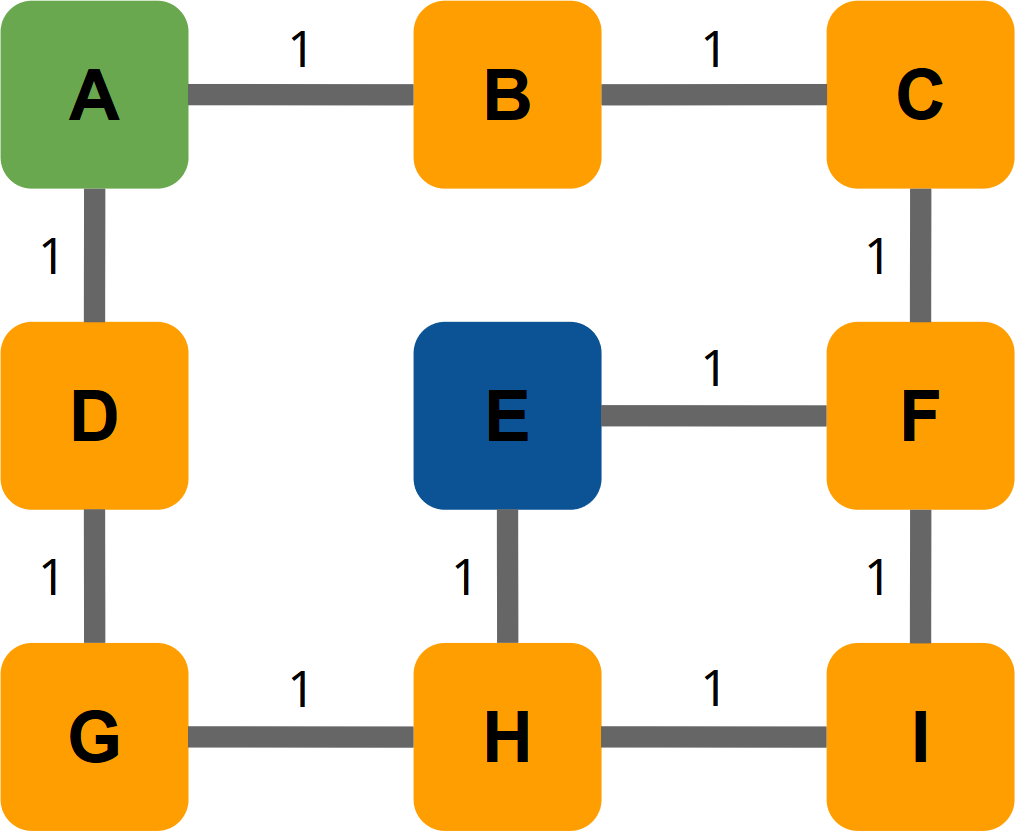
\includegraphics[width=0.7\linewidth]{sources/ex1}
	\caption{The example problem}
	\label{fig:ex1}
\end{figure}


In the beginning relevant python packages are loaded into the script.
\begin{itemize}
	\item \texttt{sys} is used, as it provides access to the \texttt{argv} array, which is filled with program parameters. This allows our script to accept problem files with different file names or locations
	\item \texttt{math} provides access to certain math operations, like \texttt{math.sqrt()} to calculate the square root of a number.
	\item \texttt{json} allows the parsing of a \texttt{json} file, which is used to define the problem.
	\item \texttt{networkx} is a graph library.\footnote{\url{https://networkx.github.io/documentation/stable/tutorial.html}} It is used to store and perform operations on the problem graph.
\end{itemize}
\begin{lstlisting}
import sys
import math
import json
import networkx as nx
\end{lstlisting}

As the next step, the program parameters are checked for a possible overwrite of the problem file name, or the program defaults into \texttt{exampleProblem.json}.
This json file is then read and the nodes and edges are added to a directed graph.

\begin{lstlisting}
# Step 1: Read input into graph
if (len(sys.argv) > 1) and (sys.argv[1] != ""):
	inputfile = sys.argv[1]
else:
	inputfile = "exampleProblem.json"
graph = nx.DiGraph()
startNode = ''
targetNode = ''
with open(inputfile) as f:
	problem = json.loads(f.read())
	for node in problem['nodes']:
	graph.add_node(node['id'], x=node['X'], y=node['Y'])
	for edge in problem['edges']:
	graph.add_edge(edge['start'], edge['end'], cost=edge['cost'])
	startNode = problem['startNode']
	targetNode = problem['targetNode']
	f.close()
\end{lstlisting}

Now two sets of nodes are initialized.
The first set, \texttt{checkedNodes} will contain nodes for which the algorithm will already have performed all operations.
This set is empty in the beginning.
The other set, \texttt{toCheckNodes} -- often also referred to as \enquote{open set} -- will contain all candidates which could contribute to a valid path.
In the beginning, this is only the node from which the search will start.
\begin{lstlisting}
checkedNodes = set()
toCheckNodes = set(startNode) # Begin with the start node
\end{lstlisting}
Additionally, each node in the graph will be supplied with values for \texttt{costToReach}, which represents the current costs to reach this node (if such a way has been found) and a \texttt{heuristic}, which will be explained in a later section.
Since the search starts at the start node, the \texttt{costToReach} value of it is set to 0.
\begin{lstlisting}
graph.nodes[startNode]['costToReach'] = 0 # cost to reach start Node is 0.
graph.nodes[startNode]['heuristic'] = calcHeuristic(startNode, targetNode)
\end{lstlisting}

After that initial setup, the main work of the algorithm happens in a loop.
As long as there are still nodes in the set \texttt{toCheckNodes}, the algorithm will keep looking for a path.
Running out of nodes to check means that all possible ways from the start node have been inspected, and since the target node has not been found, no such path can exist.

In each loop iteration, a currently most promising node is selected (see section \ref{sec:findBestNode}).
If that selected node is the target node, the path will be reconstructed and the program will end (see section \ref{sec:handlePathFound}).
Otherwise, the node's neighbors are inspected and added to the \texttt{toCheckNodes} set (see section \ref{sec:handleNeighbors}).
Finally, the node will be removed from the open set (\texttt{toCheckNodes}) and added to the set of already checked nodes, to prevent the program from performing work twice and possibly getting stuck in a infinite loop.

\begin{lstlisting}
while len(toCheckNodes) > 0: # As long as there are nodes which could lead to the target
	bestNode = findBestNode(toCheckNodes)
	
	if bestNode == targetNode:
		handlePathFound(targetNode)
	
	handleNeighbors(list(graph.neighbors(bestNode)), checkedNodes, toCheckNodes)
	
	toCheckNodes.remove(bestNode) # Node has been checked!
	checkedNodes.add(bestNode) # Node has been checked!

# No more possible nodes to lead to the target!
# I.e. there is no way to reach the target.
print('There is no route to the target.')
\end{lstlisting}

\subsection{Selection of best Node}
\label{sec:findBestNode}
As mentioned earlier, A* reaches a good performance because it has the tendency to prefer nodes which are more likely to be in the correct direction of the target node.
This is done by selecting (for the next steps) the node with the lowest \enquote{expected value}.
The \enquote{expected value} represents the (approximated) total cost of a path which leads through the node.
It is calculated as the sum of the current cost (i.e. how much was spent to arrive at a node) and the \enquote{heuristic} (i.e. how much is expected to be the cost \textit{from} this node.)
(For details about the heuristic, see section \ref{sec:calcHeuristic}.)

The best node is found simply by iterating the set of open nodes (i.e. \texttt{toCheckNodes}) and retaining those with better values.
\begin{lstlisting}
def findBestNode(toCheckNodes):
	bestNode = ''
	bestNodeScore = float("inf")
	for toCheckNode in toCheckNodes:
		score = graph.nodes[toCheckNode]['costToReach'] + graph.nodes[toCheckNode]['heuristic']
		if score < bestNodeScore:
			bestNode = toCheckNode
			bestNodeScore = score
	return bestNode
\end{lstlisting}

\subsection{Handling a detected Path}
\label{sec:handlePathFound}
Should the previously detected node be the target node, the algorithm ends, as it has found a valid path.
Since the \textit{predecessor} for every node is stored when that node is inspected (see section \ref{sec:handleNeighbors}), the path can be reconstructed by following the predecessors.

This leads to a inverse path from target to start, which then can be reversed.
Alternatively, the start and target node could have been switched at the beginning of the algorithm.
We decided to follow the first approach, as this makes the code easier to understand and the performance of our algorithm is not really affected by that.
(Reversing the list is a very cheap operation.)
\begin{lstlisting}
def handlePathFound(targetNode):
	# We arrived at the target node!
	print('=============')
	print('Found path!')
	currNode = targetNode
	path = [currNode] # We reconstruct the path backwards by following the predecessors
	while 'predecessor' in graph.nodes[currNode]:
		predecessor = graph.nodes[currNode]['predecessor']
		path.append(predecessor)
		currNode = predecessor
	path.reverse()
	print(path)
	sys.exit()
\end{lstlisting}

Such a detected path through the predecessors is shown in figure \ref{fig:path}.

\begin{figure}[H]
	\centering
	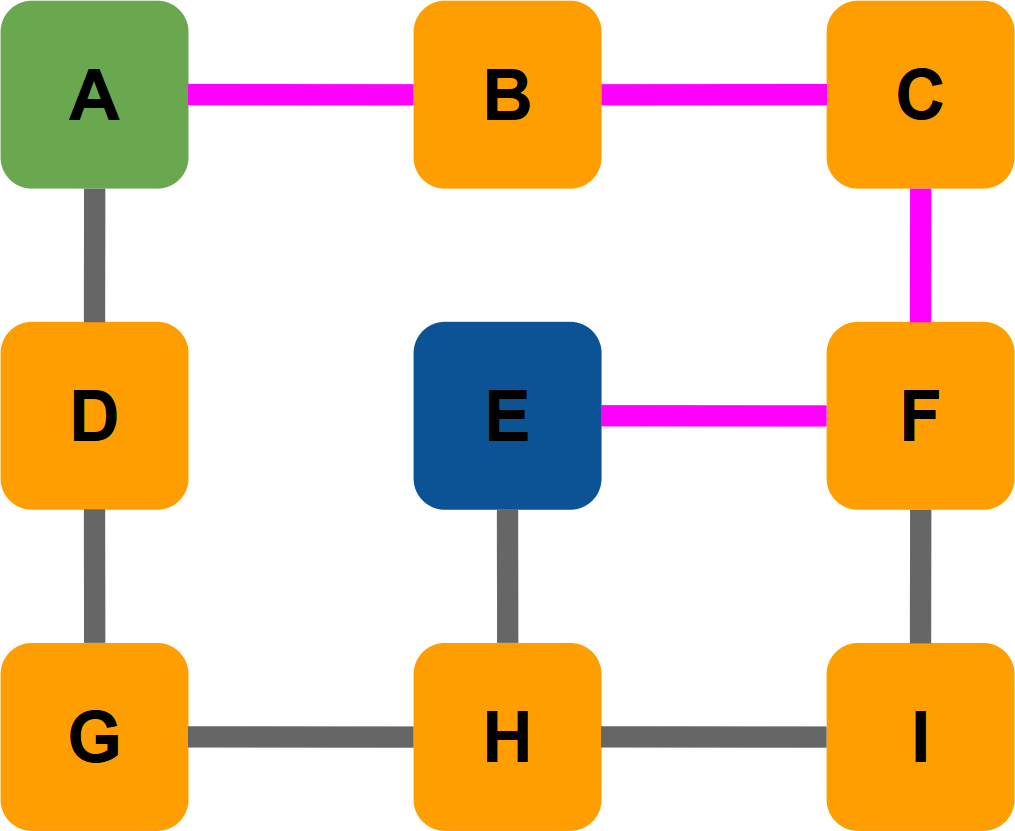
\includegraphics[width=0.7\linewidth]{sources/path}
	\caption{A found path for the example problem}
	\label{fig:path}
\end{figure}

\subsection{Inspecting Neighbors}
\label{sec:handleNeighbors}
If the selected \enquote{best node} is not the actual goal node, the neighbors of that node are inspected for possible ways to continue the path.
Node which already have been inspected are skipped.
Otherwise the node is added to the open list (i.e. \texttt{toCheckNodes}), if it is not already there. This is done, because that neighbor might continue the path to the target node.

After that a new cost for that neighbor (via the currently inspected \texttt{bestNode}) is calculated.
If it is better than that neighbor's current cost (or that neighbor does not yet have a valid path), the predecessor is set to the currently inspected node, the cost is saved and the heuristic for that neighbor is determined (see section \ref{sec:calcHeuristic}).
Otherwise, the neighbor's current predecessor and cost is kept as it is, since the new path does not provide improvement.
\begin{lstlisting}
def handleNeighbors(neighbors, checkedNodes, toCheckNodes):
	for neighbor in neighbors:
		if neighbor in checkedNodes:
			continue # We already came across this node from a better path. So we're not interested.
		if neighbor not in toCheckNodes:
			toCheckNodes.add(neighbor) # We should  check the paths going through here!
		print('New neighbor: >' + str(neighbor) + '<')
		costToGetToNeighbor = graph.nodes[bestNode]['costToReach'] + graph.edges[bestNode, neighbor]['cost']
		if 'costToReach' not in  graph.nodes[neighbor] or costToGetToNeighbor < graph.nodes[neighbor]['costToReach']:
			print('  With a better path!')
			graph.nodes[neighbor]['predecessor'] = bestNode
			graph.nodes[neighbor]['costToReach'] = costToGetToNeighbor
			graph.nodes[neighbor]['heuristic'] = calcHeuristic(neighbor, targetNode)
		else:
			print('  But the current path is already better')
\end{lstlisting}
	
The inspected neighbors after the first iteration are shown in figure \ref{fig:neighbors}. As \texttt{A} is the selected \texttt{bestNode}, both direct neighbors (detected by the connecting edges) will be updated.
\begin{figure}[H]
	\centering
	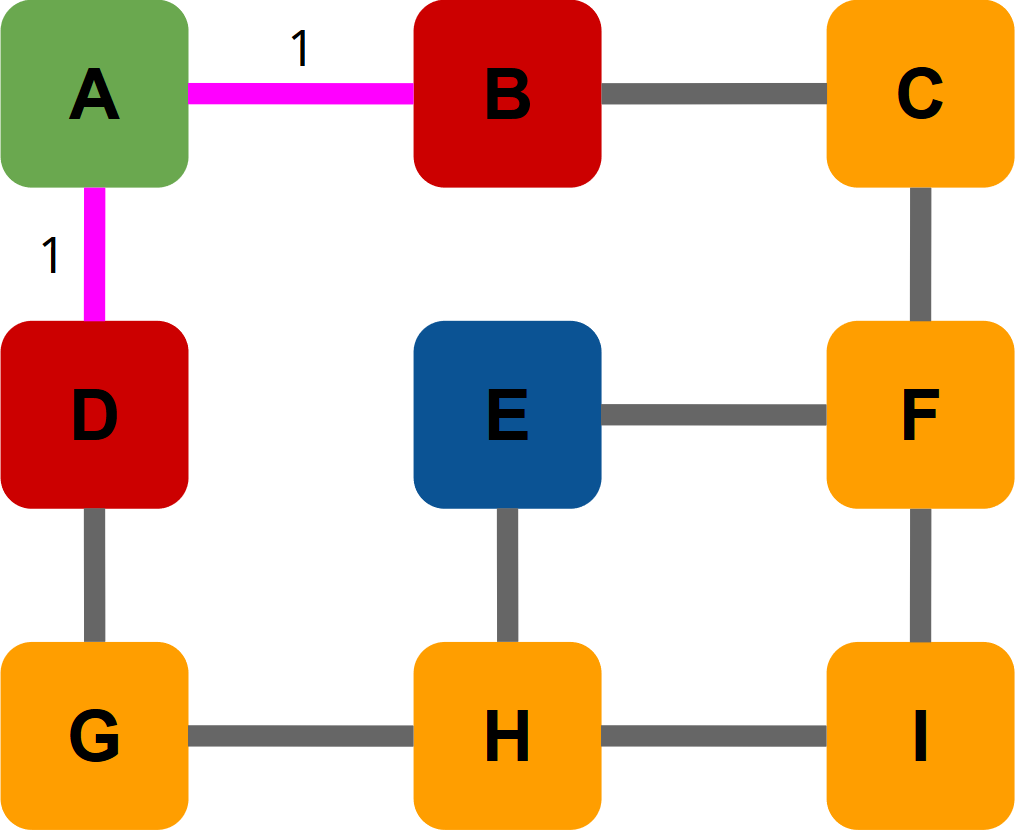
\includegraphics[width=0.7\linewidth]{sources/neighbors}
	\caption{Inspected neighbors in the example problem after the first iteration.}
	\label{fig:neighbors}
\end{figure}	

\subsubsection{Calculation of heuristic}
\label{sec:calcHeuristic}
There are many different ways to implement a heuristic (see section \ref{sec:alternativeHeuristics}).
We decided to use the euclidean heuristic with a distance-corresponding cost.
This means that two nodes which are $x$ distance unit apart, will have their most direct connection not lower than $x$ cost units.
This is a reasonable assumption for any graph that models a distance-based problem set.
I.e. the problem is only interested in finding the shortest path in distance -- the algorithm might lead to wrong results, if there were faster \enquote{roads} available. 
(E.g. in a real-live scenario it might be better to take a national road across a village, instead of the shorter-distance (but lower speed) road through the village.)

This euclidean heuristic is then simply calculated by using the pythagorean theorem to get the direct \enquote{beeline} distance between both nodes.

\begin{lstlisting}
def calcHeuristic(fromNode, toNode):
	# We assume that the cost for each edge is lower-limited by the distance between the nodes.
	# E.g. If node A is at (5|5) and node B is at (6|7), the x distance is 6-5 = 1 and the y distance is 7-5 = 2.
	# Therefore the total distance is sqrt(1^2 + 2^2) = 2.236...
	diffX = abs(graph.nodes[fromNode]['x'] - graph.nodes[toNode]['x'])
	diffY = abs(graph.nodes[fromNode]['y'] - graph.nodes[toNode]['y'])
	diffTotal = math.sqrt(diffX**2 + diffY**2)
	return diffTotal
\end{lstlisting}


\section{Alternative Heuristics}
\label{sec:alternativeHeuristics}
\todo[inline]{Saleh will do this part}


\printbibliography

%%%%%%%%%%%%%%%%%%%%%%%%%%%%
% Appendix
%%%%%%%%%%%%%%%%%%%%%%%%%%%%
\newgeometry{left=1cm, right=1cm, bottom=3cm, top=1cm, onecolumn}
\section{Appendix}
\subsection{Python code}
\label{sec:pythonCode}
\lstinputlisting{../aStar.py}



\end{document}